% ============================================================
%  OR gate - board-level wiring diagram.
%  OR has no parts of its own: it is a finished NOR board whose
%  output feeds a finished NOT board:
%        A,B -> [NOR] -> (A+B)-bar -> [NOT] -> Y = A+B
%  Build the NOR board and the NOT board, share one +5 V rail and
%  one GND, then wire them as below.
%  Compile:  pdflatex wiring.tex
% ============================================================
\documentclass[border=16pt]{standalone}
\usepackage{circuitikz}
\usepackage{tikz}
\usetikzlibrary{calc}

\begin{document}
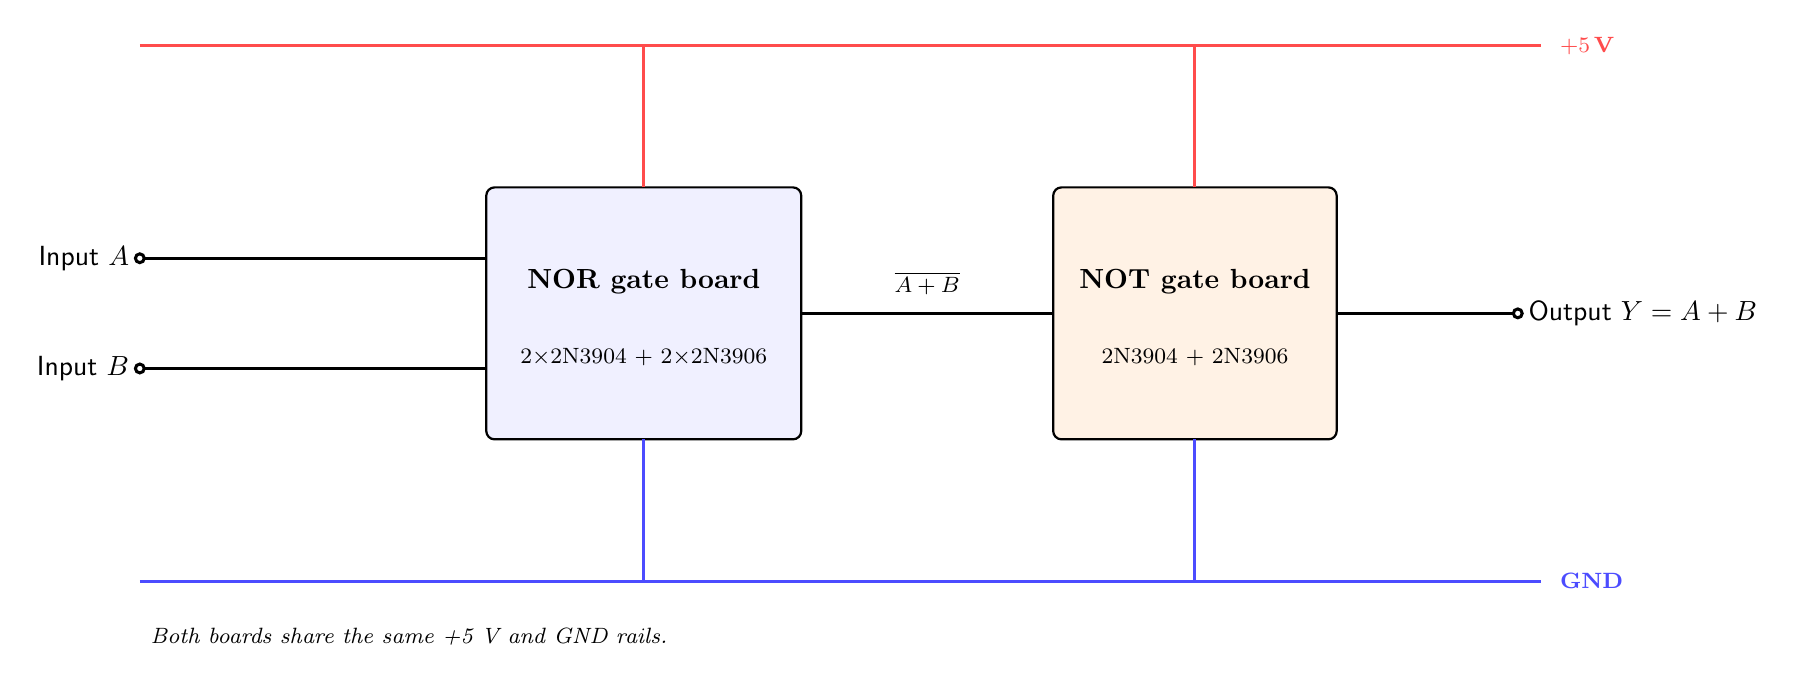
\begin{tikzpicture}[line width=1.1pt, font=\sffamily]

  % ---------- shared power rails ----------
  \draw[red!70]  (-1.8,3.4) -- (16.0,3.4);
  \node[red!70,anchor=west,font=\footnotesize\bfseries] at (16.1,3.4) {$+5\,$V};
  \draw[blue!70] (-1.8,-3.4) -- (16.0,-3.4);
  \node[blue!70,anchor=west,font=\footnotesize\bfseries] at (16.1,-3.4) {GND};

  % ---------- the two boards ----------
  \draw[thick, rounded corners=3pt, fill=blue!6] (2.6,-1.6) rectangle (6.6,1.6);
  \node[align=center, font=\bfseries] at (4.6,0.4) {NOR gate board};
  \node[align=center, font=\footnotesize] at (4.6,-0.55) {2$\times$2N3904 + 2$\times$2N3906};

  \draw[thick, rounded corners=3pt, fill=orange!10] (9.8,-1.6) rectangle (13.4,1.6);
  \node[align=center, font=\bfseries] at (11.6,0.4) {NOT gate board};
  \node[align=center, font=\footnotesize] at (11.6,-0.55) {2N3904 + 2N3906};

  % ---------- inputs A, B ----------
  \draw (-1.8,0.7) node[ocirc]{} node[left]{Input $A$} -- (2.6,0.7);
  \draw (-1.8,-0.7) node[ocirc]{} node[left]{Input $B$} -- (2.6,-0.7);

  % ---------- NOR -> NOT ----------
  \draw (6.6,0) -- (9.8,0);
  \node[above,font=\footnotesize] at (8.2,0.1) {$\overline{A+B}$};

  % ---------- output ----------
  \draw (13.4,0) -- (15.7,0) node[ocirc]{} node[right]{Output $Y=A+B$};

  % ---------- power taps ----------
  \foreach \x in {4.6,11.6}{
    \draw[red!70]  (\x,1.6) -- (\x,3.4);
    \draw[blue!70] (\x,-1.6) -- (\x,-3.4);
  }

  \node[anchor=west,font=\footnotesize\itshape] at (-1.8,-4.1)
        {Both boards share the same +5 V and GND rails.};

\end{tikzpicture}
\end{document}
